\section{Zielsetzung}
\label{sec:Zielsetzung}
In diesem Experiment werden die charakteristische Relaxationszeit $\tau_0$ und die zur Ausrichtung der Dipole nötigen Aktivierungsenergie $W$ in \ce{KBr(Sr)} ermittelt. 
\section{Theorie}
\label{sec:Theorie}
Dotierung einwertiger Ionengittern mit zweiwertigen Kationen bildet elektrische Dipole im Ionenkristall, da der Kristall nach außen hin ladungsneutral ist.
Die Dipole entstehen durch die Leerstellen und zweiwertigen Kationen.
In Abbildung \ref{fig:Dipol} ist der Sachverhalt am Beispiel von Strontiumionen (\ce{Sr^{2+}}) in Cäsiumjodid (\ce{CsJ}) zu erkennen.
\begin{figure}[htb]
  \centering
  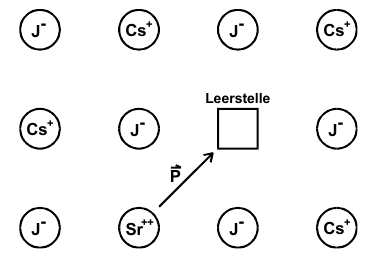
\includegraphics[height=6cm]{pics/Dipole.png}
  \caption{Mit \ce{Sr2+} dotiertes Cäsiumjodid \ce{CsJ} zur Darstellung von elektrischen Dipolen in Ionenkristallen. \cite{anleitung}}
  \label{fig:Dipol}
\end{figure}
\FloatBarrier

Die Richtung der Dipole hängt hierbei von der Verbindungsachse zwischen den Störstellen im Gitter ab, sie ist also quantisiert.
Solange die Temperatur des Kristalls unter \SI{500}{\celsius} ist, verändert sich die Dipolrichtung ausschließlich durch Leerstellendiffusion.
Dazu muss eine Potentialschwelle überwunden werden, die von dem räumlich periodischen Verlauf des Gitterpotentials abhängt.
Die nötige Energie ist die materialspezifische Aktivierungsenergie W.
Die mittlere Zeit zwischen zwei Orientierungen ist nach der Boltzmann-Statistik
\begin{equation}
    \label{eqn:Relaxzeit}
    \tau(T) = \tau_0 \exp\left(\frac{W}{\symup{k_B} T}\right)
\end{equation}
mit $\tau_0$ als charakteristische Relaxationszeit, $\symup{k_B}$ für die Boltzmann-Konstante und $T$ für die Temperatur.

Die zu untersuchende Probe dient als Dielektrikum eines Plattenkondensatoren, an dem vorerst eine Gleichspannung angelegt ist.
Durch das elektrische Feld werden einige Dipole in Feldrichtung ausgelenkt, die restlichen Dipole, wegen thermischer Gitterbausteinbewegung, zeigen
in andere Richtungen. Insgesamt zeigt also nur ein Bruchteil $y$ der Dipole in Feldrichtung.
Dieser Bruchteil lässt sich durch die Funktion
\begin{equation}
    y(T)=\frac{pE}{3\symup{k_B}T}
\end{equation}
ausdrücken.
Hierbei steht $p$ für die Dipolstärke und $E$ für die elektrische Feldstärke.

Während diese ausgerichteten Dipole wieder eine statistische Raumverteilung annehmen, was als Dipolrelaxation bezeichnet wird, ist ein Depolarisationsstrom messbar.
Der schematische Verlauf dieses Stromes ist in Abbildung \ref{fig:Strom} zu sehen.
Die Depolarisationsstromdichte ist durch
\begin{equation}
\label{eqn:Stromdichte}
    j(T)=\frac{p^2 E N_\text{p}}{3 \symup{k_B} T_\text{p}\tau_0}\exp\left(-\frac{1}{h\tau_0}\int_{T_0}^{T}\exp\left(\frac{-W}{\symup{k_B}T'}\right)d\,T'\right)\exp\left(\frac{-W}{\symup{k_B}T}\right)
\end{equation}
gegeben.
Dabei ist $T_\text{p}$ die Polarisationstemperatur, $h$ die Heizrate und $N_\text{p}$ die Zahl der zu Beginn des Aufheizens (Zeitpunkt $t_0$ und Temperatur $T_0$) vorhandenden orientierten Dipole pro Volumeneinheit.
\begin{figure}[htb]
    \centering
    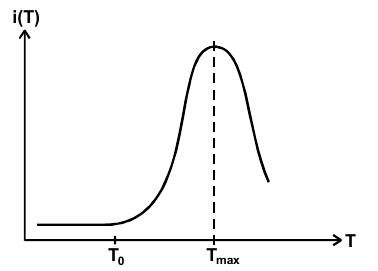
\includegraphics[height=6cm]{pics/Strom.png}
    \caption{Depolarisationsstrom in Abhängigkeit von der Temperatur. \cite{anleitung}}
    \label{fig:Strom}
\end{figure}
\FloatBarrier
Für den Anfangsteil der Depolarisationskurve genügt die Näherung
\begin{equation}
    j(T)=\frac{p^2 E N_\text{p}}{3 \symup{k_B} T_\text{p}\tau_0}\exp\left(\frac{-W}{\symup{k_B}T}\right).    
\end{equation}
Wird die Polarisation $P$ der Probe untersucht, ist es möglich $W$ genauer zu bestimmen, da der gesamte Kurvenverlauf analysiert wird.
Ist $i(t)$ der durch die Dipolrelaxation erzeugte Strom, gilt die Beziehung
\begin{equation}
    \frac{W}{\symup{k_B}T}=\ln\frac{\int_T^\infty i(T')d\,T'}{i(T)\tau_0 h}.
\end{equation}
Durch eine Regression wird $W$ schließlich ermittelt.
Die Relaxationszeit $\tau_0$ ist gegeben durch
\begin{equation}
    \label{eqn:tau0}
    \tau_0 = \frac{\symup{k_B}T_\text{max}^2}{W \cdot h} \exp\left(-\frac{W}{\symup{k_B}T_\text{max}} \right).
\end{equation}
$T_\text{max}$ ist die Temperatur bei dem der größte Strom fließt (siehe Abb. \ref{fig:Strom}). 
% \begin{figure}[htb]
%   \centering
%   \includegraphics[height=5.5cm]{content/Bild.png}
%   \caption{Bilduterschrift}
%   \label{fig:Bild}
% \end{figure}

% \subsection{Unterkapitel}
% \label{sec:UnterKapitel}

% \begin{equation}
% Für Formeln
%   \label{eqn:Formel}
% \end{equation}
\FloatBarrier